\section{Generierung von Vorschlägen für Variablen-Belegungen}\label{chap:testdatasuggestions}

%%%%%%%%%%%%%%%%
%
%   Automatische Vorschlagsgenerierung für Variablen-Belegungen
%
%%%%%%%%%%%%%%%%

%- FOKUS darauf!
%- ein gesamttestfall für kompletten algorithmus? --> Clemens
%- Testfällt updatebar machen

Um dem Entwickler repräsentative Testwerte, die die Variationspunkte eines SQL-Statements beeinflussen, vorzuschlagen, gibt es verschiedene Strategien.
Grundlage dafür bietet, wie anfangs erwähnt, ein Datenbanksystem mit den enthaltenen Echt-Daten.
In den folgenden Beispielen werden Unternehmensdaten aus einer SAP-Infrastruktur einer Aktiengesellschaft genutzt.
Die Integration solcher Datenbanksysteme und die Administration von den genutzten Test-Daten werden im Kapitel \ref{chap:testdataadministration} näher erläutert.

Neben der Betrachtung der Charakteristiken von Daten innerhalb der Datenbank, ist vor allem die Verknüpfung mit Analyse-Ergebnissen, vorrangig den Laufzeit-Messungen, ein Kriterium für die Generierung der Vorschläge.
Mittels Auswahl unterschiedlicher, vorgeschlagener Testwerte ist es dem Entwickler möglich konkrete Ausprägungen von SQL-Statements nachzuvollziehen und durch die Auswertung der Messungen gegebenenfalls Optimierungen durchzuführen bis das gewünschte Performance-Verhalten erreicht ist.


\subsection{Vorschläge auf Basis von Daten-Charakteristiken}\label{chap:datacharacteristics}
Der erste Anhaltspunkt für das Vorschlagen relevanter Testwerte ist die Charakteristik der Datenbankinhalte.
Primär spielen dabei die Verteilung der Daten innerhalb der Relationen und die Anzahl ihrer unterschiedlichen Ausprägungen eine Rolle.

%\begin{figure}
%\centering
	%\begin{tikzpicture}
		%\begin{axis}[
				%axis lines=left,
				%width  = 0.85*\textwidth,
				%height  = 6cm,
				%symbolic x coords={Males,Females},
				%xtick=data,
				%enlarge x limits=0.5,
				%bar width=40pt,
				%ybar,
				%ylabel={Percentage},
				%ymin=0.0,
				%ymax=100.0,
				%]
				%\addplot[ybar,fill=light-gray] coordinates {
						%(Males,55)
						%(Females,45)
				%};
		%\end{axis}
	%\end{tikzpicture}
	%\caption{(TODO: ersetzten durch statistik in BSEG.) Verteilung der Werte in der Spalte Gender.}
	%\label{fig:gender}
%\end{figure}

\pgfkeys{
    /pgf/number format/precision=0,
    /pgf/number format/fixed zerofill=true,
    /pgf/number format/fixed,
		/pgf/number format/.cd,
		use comma,
		1000 sep={.}
}

\begin{figure}
\centering
	\begin{tikzpicture}
		\begin{axis}[
			axis lines=left,
			xbar, xmin=0,
			width=0.85*\textwidth,
			height=6cm,
			enlarge y limits=0.1,
			xlabel={Absolute Anzahl distinkter Werte},
			symbolic y coords={MANDT,GJAHR,ZLSCH,BUKRS,AUGDT,LIFNR,SKFBT,KUNNR,WRBTR,BELNR},
			ytick=data,
			bar width=5pt,
			nodes near coords, nodes near coords align={horizontal},
			]
			\addplot[fill=light-gray] coordinates {
				(5636590,BELNR)
				(560628,WRBTR)
				(408015,KUNNR)
				(228722,SKFBT)
				(48407,LIFNR)
				(2304,AUGDT)
				(71,BUKRS)
				(31,ZLSCH)
				(10,GJAHR)
				(2,MANDT)
			};
		\end{axis}
	\end{tikzpicture}
	\caption{Verteilung distinkter Werten einer Auswahl von Spalten aus BSEG}
	\label{fig:bseg}
\end{figure}

Die Abbildung \ref{fig:bseg} zeigt eine Auswahl der 326 Spalten der BSEG-Tabelle aus einem SAP-System.
Die Tabelle enthält alle einzelnen Belegpositionen zu den Buchungsbelegen des Unternehmens.
Eine Erläuterung zu der Bedeutung der einzelnen Spalten befindet sich im Anhang (Tabelle \ref{tab:bsegerlaeuterung}).

Sollte die Anzahl der distinkten Werte einstellig sein (beispielsweise bei der Spalte MANDT), können dem Entwickler alle möglichen Ausprägungen in einem Auswahl-Menü zur Verfügung gestellt werden.
Damit wird gleichzeitig auch sichergestellt, dass nur Werte eingegeben werden können, die beim testweisen Ausführen des SQL-Statements ein Ergebnis zurückgeben.
Auf der anderen Seite können sich Spalten jedoch über eine große Menge von verschiedenen Datenausprägungen erstrecken, wie zum Beispiel bei Belegnummern (BELNR), was eine einfache Auswahl passender Testdaten kompliziert gestaltet.
Für diesen Fall werden Äquivalenzklassen anhand der Vorkommen der Werte erzeugt, die sich unterteilen in: die drei häufigste Werte, die drei seltensten Werte, drei Werte um den Median und der Rest.

Für die häufigsten Werte wird eine aufsteigende Sortierung der Anzahl des Vorkommens eines Wertes vorgenommen und die ersten drei selektiert.
Sollten mehrere Werte dieselbe Anzahl an Vorkommen vorweisen, werden sie zusätzlich anhand ihrer Werte aufsteigend sortiert.
Im Unterschied dazu wird bei der Klasse der seltensten Werten eine absteigende Sortierung vorgenommen.
Für die Werte um den Median muss zuerst die Anzahl der verschiedene Werte ermittelt werden.
Anschließend dient die Halbierung des Ergebnisses als Offset für die Bestimmung der drei Werte.
Die SQL-Statements dazu befinden sich im Anhang als Code-Beispiel \ref{lst:distinctvalues}.

Dieser Ansatz ist zum Vorschlagen einzelner Testwerte nützlich, stößt jedoch an seine Grenzen, sobald mehrere Parameter genutzt werden und diese voneinander abhängig sind.
Im Code-Beispiel \ref{lst:dynamicsql} aus dem Kapitel \ref{sec:dependencydetection} werden beispielsweise offene Rechnungen und deren Einzelposten gesucht.
Die Variable \texttt{customer} gibt dabei die Kundennummer an, mit der die Rechnungen assoziiert sind.
Sucht man nun nach der Kundennummer mit den meisten Rechnungen, bedeutet dies nicht zwangsläufig, dass man auch die mit den meisten Einzelposten oder höchsten Gesamtsummen findet.
Diese, noch recht einfache, Abhängigkeit kann beliebig erweitert werden.
Damit entstehen komplexe SQL- und Programm-Strukturen, die durch das einfache Vorschlagen anhand von Charakteristiken einzelner Spalten nicht zwangsläufig die Randfälle aufzeigen, die der Entwickler sucht.
Aus diesem Grund ist die Betrachtung von Messwerten der Analyse-Ergebnisse eine sinnvolle Erweiterung um die Genauigkeit der Vorschläge zu steigern.

\subsection{Adaptive Vorschlagsgenerierung durch Laufzeit-Analysen}\label{chap:adaptive}
Laufzeit-Analysen (\cite{Exner2014}, \cite{Mues2014}) ermöglichen das Verhalten von Datenbankzugriffen in Geschäftsanwendungen nachzuvollziehen.
Die variablen Stellen von SQL-Statements werden dabei durch die vom Entwickler ausgewählten Werte gefüllt.
Im nächsten Schritt werden nun diese atomaren Vorschläge kombiniert und mit dem dazugehörigen Ergebnis aus der Laufzeit-Analyse verknüpft.
Dies ermöglicht Vergleichbarkeit verschiedener Konstellationen.
Für die Erstellung der initialen Daten können zwei verschiedene Ansätze verfolgt werden.

Mithilfe der Brute-Force-Methode können alle Kombinationen durchprobiert und gemessen werden.
Der enorme Aufwand, gerade bei besonders Relationen mit vielen Einträgen und distinkten Werten in den Spalten, stellt jedoch aufgrund der enormen Berechnungszeit ein großes Hindernis dar.

Dem gegenüber steht der adaptive Ansatz, bei dem der Testdaten-Bestand kontinuierlich erweitert wird.
Diese Variante speichert die Ergebnisse der Laufzeit-Analysen mit den dazugehören Testdaten-Konstellationen als Testdaten-Sets.
Sobald mehrere dieser Sets vorhanden sind, können dem Entwickler drei Vorauswahl-Optionen gegeben: das Testdaten-Set mit der höchsten Laufzeit, mit der geringsten Laufzeit und mittlerer Laufzeit.

Um für diese Methode eine Datengrundlage zu schaffen, werden die in Kapitel \ref{chap:datacharacteristics} ermittelten Werte genutzt um initiale Kombinationen zu bilden und ihre Laufzeiten zu berechnen.
Durch Eingabe weiterer Werte durch den Entwickler kann anschließend das Datenmodell kontinuierlich erweitert und zunehmend verbessert werden, zu sehen im Code-Beispiel \ref{lst:developerinput}.

\begin{lstlisting}[caption={Eingaben von Testwert-Konstellationen erweitern gegebenenfalls das Datenmodell}, label={lst:developerinput}, language=Python]
	hier
	kommt
	der
	algorithmus
	rein
\end{lstlisting}

TODO: Algorithmus beschreiben.

\subsection{Betrachtung von Zeitbereichsanfragen}
Ein typischer Bestandteil von Datenbankanfragen in Geschäftsanwendungen sind Bereichsfilter mittels \texttt{column BETWEEN x AND y},  insbesondere für Zeiträume.
Der in Kapitel \ref{chap:datacharacteristics} vorgestellte Algorithmus generiert Vorschläge basierend auf binären Operationen (zumeist Vergleiche), wohingegen ein Bereichsfilter ternär ist.
Deshalb ist eine besondere Betrachtung für passende Vorschläge sinnvoll.

Sollte eine Bereichsanfrage erkannt werden, die eine Spalte vom Datentyp \texttt{DATE} referenziert, so kann der Entwickler eine vorgeschlagene Zeitraumgröße (z.B. eine Woche, ein Monat oder ein Jahr) auswählen oder selbst festlegen.
Anschließend wird die referenzierte Spalte mithilfe der angegebenen Zeitraumgröße gescannt, ähnlich dem Prinzip des Sliding Window\footnote{\url{http://en.wikipedia.org/wiki/Sliding_window_protocol}}.
Auf dieser Basis werden, ähnlich dem Algorithmus aus Kapitel \ref{chap:datacharacteristics}, bis zu 3 Vorschläge für die größte, kleinste und mittlere Anzahl an Resultaten erzeugt.
Alternativ steht es dem Entwickler offen, Start- und Enddatum eigenständig festzulegen.

\subsection{Integration in die IDE}
\begin{figure}[ht]
	\centering
  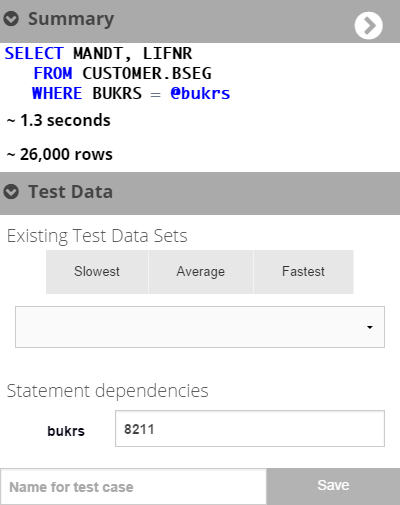
\includegraphics[width=0.4\textwidth]{figures/integration.png}
	\caption{Einbindung der Vorschläge in die Sidebar der Web-IDE}
	\label{fig:ideintegration}
\end{figure}

Die in Kapitel \ref{chap:datacharacteristics} und \ref{chap:adaptive} erzeugten Vorschläge werden in der zur Web-IDE gehörenden Datenbank gespeichert und in einer Sidebar im Frontend eingebunden (vgl. Abbildung \ref{fig:ideintegration}).
Durch das Auswählen des Entwicklers einer Quelltext-Zeile mit SQL-Inhalt, werden die Informationen zu dem dazugehörigen SQL-Statement aggregiert und aufbereitet (vgl. Kapitel \ref{chap:entwicklungsumgebung}) und schließlich in der Sidebar angezeigt.

TODO: Betrachtung vom AST?

Aus der im Kapitel \ref{chap:adaptive} ermittelten Menge an Testdaten-Sets werden zum einen die drei mit der höchsten, geringsten und durchschnittlichen Laufzeit angeboten, zum anderen ein Auswahl-Menü mit allen gespeicherten Sets.
Die Auswahl einer dieser Optionen füllt die Eingabefelder für die Testdaten automatisch mit den gespeicherten Werten und löst eine Analyse aus.
Möchte der Entwickler weitere Testdaten-Sets hinzufügen, so kann er diese benennen und direkt abspeichern.
Die Verwaltung dieser gespeicherten Daten wird im folgenden Kapitel behandelt.

\subsubsection{Nutzung von Meta-Informationen für UI-Elemente}
Um den Entwickler bei der Eingabe von Testdaten zu unterstützen, können Meta-Informationen über die Relationen genutzt werden.
Dazu kann der Datentyp von Spalten einer Relation für die Erstellung der Eingabefelder genutzt werden kann.
Beispielweise kann die Eingabe, die eine Spalte mit Datumsangaben referenziert, durch einen Kalender vereinfacht werden.
Auch die Einschränkung auf Datentypen, z.B. Ganzzahlen, kann fehlerhafte Eingabe durch den Entwickler verhindern.
Eine weitere Unterstützung ist die Autovervollständigung von teilweise eingegeben Werten.
Mittels des SQL-Operators \texttt{LIKE} kann dafür nach Daten gesucht werden, die dem Muster der bisherigen Eingabe entsprechen.